\scanpage{9}
% The printed face is read after a half turn.
% letterhead
\figure{
\begin{tikzpicture}[x=.23cm,y=.23cm]
\fill (0,.18) circle (.18);
\fill (-.05,1.13)--(-.23,1.03)--(-.23,.56)--(-.49,.81)--(-.64,.71)--(-.31,.37)
 .. controls (-.20,.28) and (-.05,.34) .. (-.05,.48)--cycle;
\fill (.05,1.13)--(.23,1.03)--(.23,.56)--(.49,.81)--(.64,.71)--(.31,.37)
 .. controls (.20,.28) and (.05,.34) .. (.05,.48)--cycle;
\fill (-.69,.67)--(-.76,.49)--(-.50,.24)--(-.88,.24)--(-.93,.04)--(-.39,.04)
 .. controls (-.20,.05) and (-.17,.19) .. (-.28,.30)--cycle;
\fill (.69,.67)--(.76,.49)--(.50,.24)--(.88,.24)--(.93,.04)--(.39,.04)
 .. controls (.20,.05) and (.17,.19) .. (.28,.30)--cycle;
\end{tikzpicture}}
\begin{center}\textsf{\textbf{CREDIT LYONNAIS}}\end{center}

\begin{flushright}Janvier 1978\\\end{flushright}

\noindent Madame, Mademoiselle, Monsieur,\\

Vous êtes titulaire d'un compte au Crédit Lyonnais. Utilisez-le, si ce n'est déjà fait, pour simplifier vos paiements et mieux contrôler vos dépenses, en demandant par exemple à bénéficier du ``prélèvement automatique'' des factures EDF - GDF.

Le ``prélèvement automatique'' est un service, entièrement gratuit, qui vous libère du souci d'effectuer vous-même le règlement de vos factures et vous évite le risque d'oubli ou de retard, même en cas d'absence prolongée de votre domicile.

Quelques jours avant chaque prélèvement, vous recevez votre facture d'électricité et de gaz, qui indique clairement le montant du prélèvement et la date à laquelle il doit être effectué. Vous disposez ainsi d'un délai suffisant pour provisionner votre compte si cela est nécessaire, ou, en cas de désaccord sur le montant de la facture, pour faire suspendre le prélèvement correspondant, sur simple demande à notre Agence ou aux services locaux d'EDF - GDF.

En outre, si malencontreusement, un prélèvement ne pouvait être effectué en raison d'une insuffisance de provision de votre compte, EDF - GDF vous demanderait de bien vouloir régler votre facture par tout autre moyen à votre convenance.

Enfin, vous avez toujours la possibilité d'annuler ce mode de paiement auprès des services locaux d'EDF - GDF.

Nous vous prions de croire, Madame, Mademoiselle, Monsieur, à l'assurance de nos sentiments distingués.\\

\begin{flushright}Le Crédit Lyonnais\\\end{flushright}

% printed form
\noindent\fcolorbox{black}{black!8}{\begin{minipage}{.94\linewidth}
Pour adopter la formule de ``prélèvement automatique'', il vous suffit de :
\begin{itemize}[label=--,leftmargin=1em,nosep]
\item compléter l'``autorisation de prélèvements'' ci-dessous ; vous trouverez les informations nécessaires :
\begin{itemize}[label=--,leftmargin=1em,nosep]
\item pour la partie A, sur votre extrait de compte,
\item pour la partie B, sur votre dernière facture EDF - GDF ;
\end{itemize}
\item envoyer ou remettre cette ``autorisation de prélèvements'', ACCOMPAGNÉE D'UN RELEVÉ D'IDENTITÉ BANCAIRE (à détacher de votre extrait de compte) à l'Unité d'exploitation EDF - GDF dont vous avez relevé l'adresse sur votre facture.
\end{itemize}
\begin{center}\rule{.24\linewidth}{.3pt}\end{center}
Il se peut que, dans votre commune, l'électricité ou le gaz ne soient pas distribués par EDF ou GDF. Nous vous demandons, dans ce cas, de vous rapprocher de notre agence ou des services locaux de votre fournisseur d'électricité ou de gaz.
\end{minipage}}

\figure{\begin{tikzpicture}[x=.16cm,y=.16cm,line cap=round]
\draw[dash pattern=on 9pt off 3pt] (-.55,0)--(58,0);
\draw[thick] (.01,.30) .. controls (-1.09,1.08) and (-.96,.00) .. (-.08,.14)
 .. controls (.04,.15) and (.17,.26) .. (.01,.30) -- (.56,-.15)
 .. controls (1.60,-.67) and (2.28,-.84) .. (2.43,-.76) -- (.51,.20) -- (.08,.18);
\draw[thick] (.01,-.30) .. controls (-1.09,-1.08) and (-.96,.00) .. (-.08,-.14)
 .. controls (.04,-.15) and (.17,-.26) .. (.01,-.30) -- (.56,.15)
 .. controls (1.60,.67) and (2.28,.84) .. (2.43,.76) -- (.51,-.20) -- (.08,-.18);
\fill (.55,0) circle (.04);
\end{tikzpicture}}

% printed form
\noindent\begin{minipage}[t]{.66\linewidth}\sffamily
AUTORISATION DE PRÉLÈVEMENTS

J'autorise le Crédit Lyonnais à débiter le montant de mes factures EDF - GDF Services nationaux, sur mon compte, si l'avoir est suffisant et sauf opposition de ma part.
\end{minipage}\hfill
\begin{minipage}[t]{.30\linewidth}\centering\small\sffamily
\begin{tabular}{|c|}\hline
Numéro national d'émetteur\\\hline
00 1007\\\hline
\end{tabular}
\end{minipage}

\figure{\resizebox{\linewidth}{!}{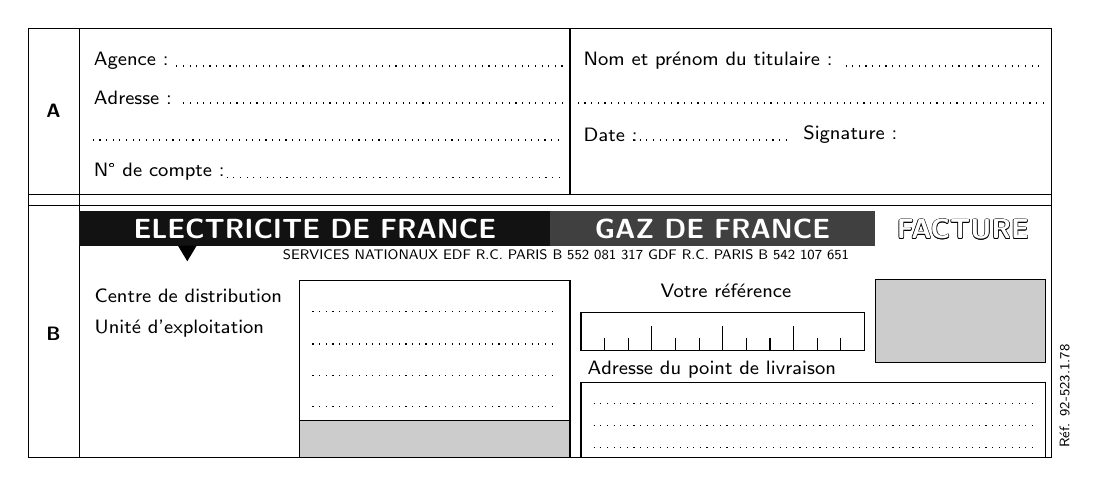
\begin{tikzpicture}[x=1cm,y=1cm,font=\sffamily\scriptsize]
\draw (0,0) rectangle (13,5.45);
\draw (.65,0)--(.65,5.45) (0,3.34)--(13,3.34) (0,3.20)--(13,3.20)
 (6.88,3.34)--(6.88,5.45);
\node at (.32,4.4) {\textbf{A}};
\node[anchor=west] at (.71,5.04) {Agence :}; \draw[dotted] (1.88,4.97)--(6.79,4.97);
\node[anchor=west] at (.71,4.57) {Adresse :}; \draw[dotted] (1.97,4.50)--(6.79,4.50);
\draw[dotted] (.82,4.03)--(6.79,4.03);
\node[anchor=west] at (.71,3.63) {N° de compte :}; \draw[dotted] (2.52,3.55)--(6.79,3.55);
\node[anchor=west] at (6.93,5.04) {Nom et prénom du titulaire :};
\draw[dotted] (10.38,4.97)--(12.89,4.97) (6.98,4.50)--(12.91,4.50);
\node[anchor=west] at (6.93,4.10) {Date :};
\draw[dotted] (7.68,4.03)--(9.69,4.03);
\node[anchor=west] at (9.72,4.10) {Signature :};
\node at (.32,1.57) {\textbf{B}};
\fill[black!93] (.65,2.69) rectangle (6.63,3.13);
\fill[black!75] (6.63,2.69) rectangle (10.75,3.13);
\node[text=white,font=\sffamily\bfseries] at (3.64,2.90) {ELECTRICITE DE FRANCE};
\node[text=white,font=\sffamily\bfseries] at (8.69,2.90) {GAZ DE FRANCE};
\foreach \dx/\dy/\ink in {-.22/0/black,-.16/.16/black,0/.22/black,.16/.16/black,.22/0/black,.16/-.16/black,0/-.22/black,-.16/-.16/black,0/0/white}{
  \node[xshift=\dx pt,yshift=\dy pt,text=\ink,font=\sffamily\bfseries] at (11.87,2.90) {FACTURE};
}
\fill (1.90,2.69)--(2.02,2.49)--(2.14,2.69)--cycle;
\node[font=\sffamily\tiny] at (6.83,2.57) {SERVICES NATIONAUX EDF R.C. PARIS B 552 081 317 GDF R.C. PARIS B 542 107 651};
\node[anchor=west] at (.72,2.05) {Centre de distribution};
\node[anchor=west] at (.72,1.63) {Unité d'exploitation};
\fill[black!20] (3.45,0) rectangle (6.88,.47);
\draw (3.45,0) rectangle (6.88,2.25) (3.45,.47)--(6.88,.47);
\foreach \y in {1.85,1.44,1.04,.65}{\draw[dotted] (3.61,\y)--(6.72,\y);}
\node at (8.86,2.11) {Votre référence};
\draw (7.02,1.36) rectangle (10.62,1.84);
\foreach \x in {7.32,7.62,8.22,8.52,9.12,9.42,10.02,10.32}{\draw (\x,1.36)--(\x,1.51);}
\foreach \x in {7.92,8.82,9.72}{\draw (\x,1.36)--(\x,1.67);}
\filldraw[fill=black!20] (10.76,1.20) rectangle (12.92,2.26);
\node[anchor=west] at (6.98,1.11) {Adresse du point de livraison};
\draw (7.02,0) rectangle (12.92,.95);
\foreach \y in {.68,.40,.12}{\draw[dotted] (7.18,\y)--(12.80,\y);}
\node[rotate=90,anchor=west,font=\sffamily\tiny] at (13.16,.00) {Réf. 92-523.1.78};
\end{tikzpicture}}}

En cas de désaccord sur le montant d'un prélèvement, je réglerai le différend directement avec EDF-GDF.

Il est entendu qu'aucun avis particulier ne me sera adressé lors de l'exécution, ou, éventuellement, de la non-exécution des prélèvements.

\begin{flushright}\small 3420\\\end{flushright}
\figure{\makebox[\linewidth][r]{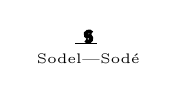
\begin{tikzpicture}[x=.19cm,y=.19cm]
\draw[line width=1.4pt] (.61,.75) .. controls (.46,.98) and (.10,.81) .. (.21,.57)
 .. controls (.30,.35) and (.48,.76) .. (.56,.43)
 .. controls (.62,.22) and (.33,.07) .. (.18,.27);
\draw (-.52,.04)--(.97,.04);
\node[anchor=north,font=\tiny] at (.36,.02) {\unsure{Sodel|Sodé}};
\end{tikzpicture}}}
% archive sheet number: 8
